{ %section1_3
	\subsection{Classification of parallel systems (architectures)}
	\par By physical architecture, parallel systems can be divided into 2 types:
		\begin{enumerate}
			\item\textbf{SMP} (Shared Memory Parallelism, Symmetric MultiProcessor system)~-- multiprocessing, multicore, GPGPU. 
			\item\textbf{MPP} (Massively Parallel Processing) -- cluster systems, GRID (distributed computing).
		\end{enumerate}
	\par We consider these two architectures in more detail.
	\par\textbf{\textit{SMP}} –- architecture of multiprocessor systems in which two or more identical processors of comparable performance are connected in the same way to the shared memory (and peripheral devices) and perform the same functions (why, in fact, the system is called symmetrical). SMP systems are also called tightly coupled multiprocessors, since in this class of systems processors are closely connected to each other via a common bus and have equal access to all resources of the computing system (memory and input-output devices) and are controlled by all one copy of the operating system. In this architecture, all processors are located on the same physical machine, so they have common memory banks. There are two types of connecting processors to shared memory:
		\begin{itemize}
			\item The connection on the system bus is shown in the Figure~\ref{SMPSystemBus:image}. In this case, only one processor can access memory at any given moment, which imposes a significant limitation on the number of processors supported in such systems. The more processors, the greater the load on the shared bus, the longer each processor must wait until the bus is free to access the memory. A decrease in the overall performance of such a system with an increase in the number of processors occurs very quickly, therefore, usually in such systems the number of processors does not exceed 2-4. An example of SMP machines with this method of connecting processors is any entry-level multiprocessor server.
				\begin{figure}[H]
					\includegraphics[width=1\linewidth]{SMPSystemBus}
					\caption{\textit{SMP architecture. Processor connection via system bus}}
					\label{SMPSystemBus:image}
				\end{figure}
			\item The crossbar switch is shown in the Figure~\ref{SMPCrossbarSwitch:image}. With this connection, the entire shared memory is divided into memory banks, each memory bank has its own bus, and the processors are connected to all buses, having access to any of the memory banks through them. Such a connection is technologically more complex, but it allows processors to access shared memory at the same time. This allows you to increase the number of processors in the system to 8-16 without a noticeable decrease in overall performance.
				\begin{figure}[H]
					\includegraphics[width=1\linewidth]{SMPCrossbarSwitch}
					\caption{\textit{SMP architecture. Processor connection via dial-up connection}}
					\label{SMPCrossbarSwitch:image}
				\end{figure}
		\end{itemize}
	\par The advantages of this approach are the high speed of data exchange between processors and the relative simplicity of software development. However, there may be problems with the scalability of the system (if there are only 2 sockets on the motherboard, you can’t put 3 processors anymore).
	\par\textbf{\textit{MMP}} -- architecture of multiprocessor systems, in which the memory between the processors is physically divided. On such systems, distributed computing is performed. The system is built from separate nodes containing a processor, a local memory bank, communication processors or network adapters, sometimes hard drives and other input-output devices. Access to the memory bank of this node is available only to processors from the same node. The nodes are connected by special communication channels (Figure~\ref{MMP:image}).
		\begin{figure}[H]
			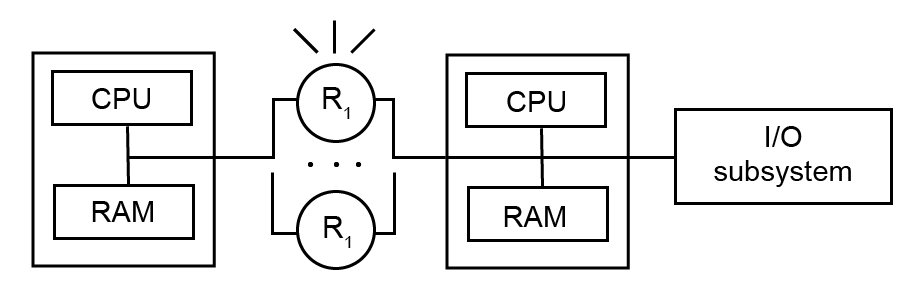
\includegraphics[width=1\linewidth]{MMP}
			\caption{\textit{MMP Architecture}}
			\label{MMP:image}
		\end{figure}
	\par The advantages of this approach are its good scalability (if necessary, to increase system performance it is enough to simply add more nodes). However, the speed of interprocessor exchange is significantly reduced, since memory banks are now physically separated. Also, the cost of the software that distributes the calculations is very high.
	\par
}
